\section{System time constant}
\label{sec:WT_TimeConstant}

\subsection*{Purpose:}
The purpose of this test is to determine the time constant and settling time of the water distribution network.


%\subsection{One clamp push} % \label{app:...}
\subsection*{Test equipment:}
\begin{itemize}
\item The water distribution system at AAU [AAU No: 100911]
\end{itemize}

\subsection*{Procedure:}
The following procedure was made for finding the time constant:
\begin{enumerate}
\item Wait for the system to get into a steady state position with the following system setup: valve opening at $0.7 \%$ for all consumer valves and differential pressure over pumps at $C2 = C16 = 0.2$[bar], $C18 = 0.1 $[bar], $C25 = 0.25$[bar].
\item Increase the differential pressure over C2 with 0.1[bar].
\item Wait 1.5 hour for the level in the WT to settle.
\end{enumerate}


\subsection*{Measuring data:}
The measurements data can be found on the attached storage under the path: \path{CD:/Data/WT timeconstant}, a plot of the data is shown in \figref{fig:Test_WT_Timeconstant}.

\subsection*{Results:}

The time constant of the system can be found through the linear differential equation shown in \eqref{statespace_4}. By Laplace transform and solving for the input output relation, the standard form of the transfer function for the system can be derived as see in \eqref{eq:std_trans_tank_time}

\begin{equation}
	\begin{split}
	&\Delta \dot{p}_{wt} = A_p \Delta \hat{p}_{wt}  + \pmb{B_p}\pmb{\hat{u}}\\
	&s\Delta p_{wt}(s) = A_p \Delta \hat{p}_{wt}(s)  + \pmb{B_p}\pmb{\hat{u}(s)}\\
	&\frac{\Delta p_{wt}(s)}{u(s)} = \frac{B}{s-A} = \frac{\frac{B}{A}}{\frac{1}{A}s + 1}
	\end{split}
	\label{eq:std_trans_tank_time}
\end{equation}

From the denominator, the time constant of the system can be directly read as seen in \eqref{eq:direct_time_constant}

\begin{equation}
	\tau s + 1
	\label{eq:direct_time_constant}
\end{equation}

 Since A in \eqref{statespace_4} is a scalar, due to the first order model only having one state, the system has one time constant. 

As the dynamics of the water distribution network are described by a first order system, the time constant can be found as the time the system uses to reach $63.2\%$ of the steady state pressure.
This pressure at $63.2\%$ of the steady state values is based on the minimum and maximum pressure values during the step and determined to:

\begin{equation}
(0.137 - 0.127)\cdot63.2 \% = 0.0063 \rightarrow 0.127 + 0.0063 = 0.133 \unit{bar} 
\end{equation}

Based on the data is it determined that at a pressure of 0.133 bar has 1155 seconds passed which corresponds to 19,25 minutes, thus the time constant is determined. 
On \figref{fig:Test_WT_Timeconstant} the measurement data used to determine the time constant of the WT is shown. A small red dot indicates the time constant for the tank.

\begin{figure}[H]
% This file was created by matlab2tikz.
%
%The latest updates can be retrieved from
%  http://www.mathworks.com/matlabcentral/fileexchange/22022-matlab2tikz-matlab2tikz
%where you can also make suggestions and rate matlab2tikz.
%
\definecolor{mycolor1}{rgb}{0.00000,0.44700,0.74100}%
%
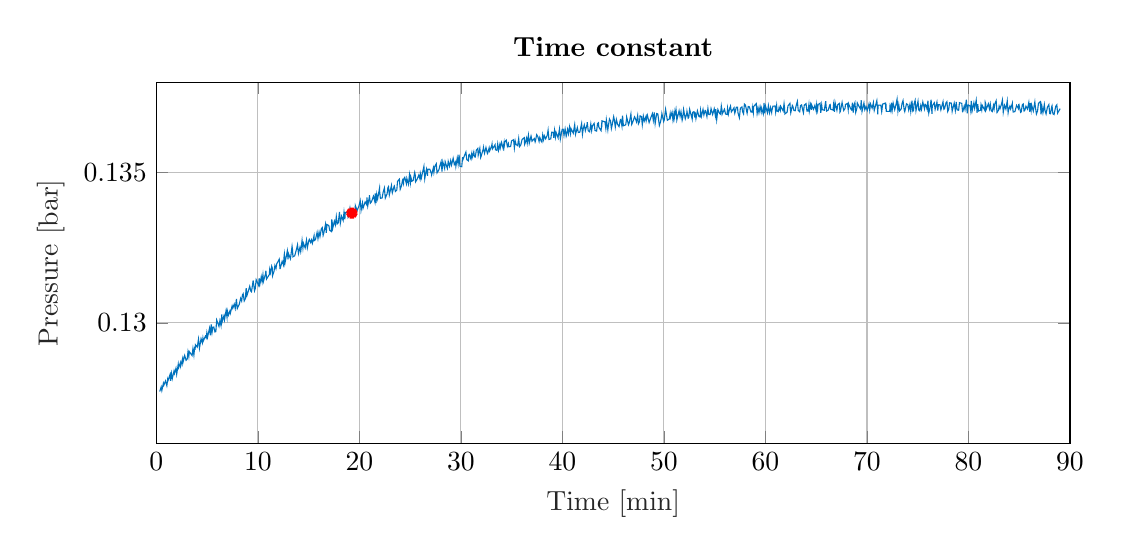
\begin{tikzpicture}

\begin{axis}[%
width=4.568in,
height=1.803in,
at={(0.766in,0.486in)},
scale only axis,
xmin=0,
xmax=90,
xlabel style={font=\color{white!15!black}},
xlabel={Time [min]},
ymin=0.126,
ymax=0.138,
ylabel style={font=\color{white!15!black}},
ylabel={Pressure [bar]},
yticklabel style={/pgf/number format/.cd,fixed,precision=3},
axis background/.style={fill=white},
title style={font=\bfseries},
title={Time constant},
xmajorgrids,
ymajorgrids
]
\addplot [color=mycolor1, forget plot]
  table[row sep=crcr]{%
0.332499999999996	0.127718914956006\\
0.473333333333329	0.127870293255128\\
0.538333333333327	0.127749364613877\\
0.691666666666663	0.127992961876828\\
0.74166666666666	0.12793119257087\\
0.894166666666663	0.128068651026396\\
1.03083333333333	0.127909442815252\\
1.11416666666666	0.128131290322585\\
1.15166666666667	0.128088660801566\\
1.34333333333333	0.128282668621708\\
1.38583333333334	0.128073870967739\\
1.48	0.128322688172048\\
1.56416666666667	0.128142600195503\\
1.73333333333333	0.128398377321602\\
1.78583333333333	0.128318338220922\\
1.92833333333333	0.128489726295214\\
1.99916666666667	0.128293108504394\\
2.15333333333334	0.128623704789845\\
2.19166666666666	0.128509736070384\\
2.37166666666667	0.128676774193551\\
2.395	0.128563675464335\\
2.57916666666667	0.128808142717503\\
2.59916666666666	0.128657634408611\\
2.78666666666666	0.128916891495606\\
2.92583333333333	0.128753333333336\\
3.03166666666667	0.128791612903228\\
3.11333333333333	0.129037820136858\\
3.19583333333334	0.128879481915931\\
3.24083333333333	0.129044780058649\\
3.51666666666667	0.128913411534711\\
3.60083333333333	0.129144828934514\\
3.69500000000001	0.128929071358741\\
3.77833333333334	0.12920833822092\\
3.81	0.129100459433047\\
3.8475	0.12927184750734\\
4.02500000000001	0.129193548387093\\
4.15000000000001	0.129460635386124\\
4.24166666666666	0.129156138807431\\
4.40083333333334	0.12947455522972\\
4.52666666666667	0.129333616813312\\
4.58416666666666	0.129491085043995\\
4.625	0.129398866080166\\
4.82833333333333	0.129556334310863\\
4.90916666666666	0.129502394916912\\
4.97083333333333	0.129668563049862\\
5.03749999999999	0.129520664711634\\
5.235	0.129822551319648\\
5.31833333333333	0.129589393939384\\
5.40083333333334	0.129951309872922\\
5.4825	0.129683352883674\\
5.56333333333333	0.129859090909093\\
5.65833333333333	0.129862570870003\\
5.7675	0.129699012707718\\
5.8575	0.129711192570866\\
5.94	0.130098338220932\\
6.16500000000001	0.129883450635404\\
6.26000000000001	0.130079198435965\\
6.36416666666666	0.129915640273708\\
6.44750000000001	0.130286256109471\\
6.47499999999999	0.130033958944281\\
6.65166666666667	0.1302349266862\\
6.70916666666666	0.130102688172059\\
6.86166666666666	0.130407184750723\\
6.95666666666666	0.130193167155426\\
6.99250000000001	0.130397614858254\\
7.09333333333333	0.130256676441832\\
7.23916666666666	0.130393264907141\\
7.28416666666666	0.130321055718468\\
7.46083333333334	0.130566392961882\\
7.5275	0.130488963831866\\
7.66833333333334	0.13062468230693\\
7.76916666666666	0.130478523949179\\
7.88916666666667	0.130796070381237\\
7.895	0.130752570870001\\
7.97	0.130481133919858\\
8.15666666666667	0.130610762463334\\
8.30333333333334	0.130820430107519\\
8.40000000000001	0.130729951124152\\
8.47583333333334	0.130930048875854\\
8.54916666666666	0.130970068426208\\
8.65166666666667	0.130730821114398\\
8.76083333333334	0.13080390029323\\
8.84333333333333	0.131157116324545\\
8.91833333333334	0.130907429129991\\
9.11333333333333	0.131124056696009\\
9.19500000000001	0.131219755620705\\
9.30666666666667	0.131050977517106\\
9.36916666666667	0.131033577712614\\
9.53	0.131405933528811\\
9.53083333333333	0.131416373411511\\
9.66916666666667	0.131068377321597\\
9.73583333333333	0.131133626588465\\
9.82916666666667	0.131437253176955\\
10.0841666666667	0.131238025415442\\
10.1191666666667	0.131484232649086\\
10.2025	0.131298924731198\\
10.3308333333333	0.131537302052763\\
10.4141666666667	0.131369393939352\\
10.4975	0.131599941348981\\
10.5525	0.131387663734131\\
10.755	0.131637350928642\\
10.7866666666667	0.131740879765388\\
10.85	0.131458132942342\\
11.1216666666667	0.131607771260988\\
11.165	0.131782639296162\\
11.2408333333333	0.131666060606065\\
11.3591666666667	0.13188790811337\\
11.415	0.131827008797629\\
11.4425	0.131565141739955\\
11.59	0.131720869990218\\
11.6733333333333	0.131909657868988\\
11.7791666666667	0.131805259042039\\
11.8558333333333	0.131961857282491\\
12.1008333333333	0.132121065493635\\
12.1841666666667	0.131787859237534\\
12.1866666666667	0.131800039100668\\
12.3891666666667	0.132049726295179\\
12.5158333333333	0.131927927663725\\
12.5908333333333	0.1322567839687\\
12.605	0.132289843597249\\
12.6625	0.131982737047906\\
12.8991666666667	0.132395112414457\\
12.9691666666667	0.132116715542509\\
13.01	0.132309853372448\\
13.2083333333333	0.132134985337231\\
13.3658333333333	0.132547360703811\\
13.4125	0.132431652003902\\
13.4491666666667	0.13219849462368\\
13.625	0.132232424242446\\
13.7908333333333	0.132437741935462\\
13.9025	0.132599560117285\\
13.9958333333333	0.132309853372448\\
14.14	0.132507341153485\\
14.2175	0.132371622678392\\
14.2341666666667	0.132411642228732\\
14.3525	0.13274919843596\\
14.4358333333333	0.13249690127077\\
14.4841666666667	0.132652629521019\\
14.6583333333333	0.132493421309846\\
14.7891666666667	0.132757028347996\\
14.8725	0.132500381231694\\
15.0183333333333	0.132742238514169\\
15.0641666666667	0.132777908113411\\
15.1966666666667	0.132675249266839\\
15.28	0.132759638318674\\
15.3641666666667	0.132647409579704\\
15.53	0.132896226783956\\
15.5541666666667	0.132739628543476\\
15.665	0.132764858260003\\
15.8316666666667	0.133011935483879\\
15.9191666666667	0.132806617790806\\
16.0275	0.133022375366551\\
16.1158333333333	0.132876217008786\\
16.2516666666667	0.133133734115347\\
16.3408333333333	0.13317114369498\\
16.4241666666667	0.132911016617797\\
16.49	0.132985835777163\\
16.6608333333333	0.133281632453603\\
16.7383333333333	0.132994535679344\\
16.7991666666667	0.133274672531797\\
16.9858333333333	0.133239872922815\\
17.0716666666667	0.133081534701887\\
17.2333333333333	0.133042385141735\\
17.2791666666667	0.133443450635411\\
17.315	0.133367761485829\\
17.3633333333333	0.133138084066445\\
17.5325	0.133385161290363\\
17.6291666666667	0.133260752688201\\
17.725	0.133538279569891\\
17.8091666666667	0.13329294232652\\
17.9158333333333	0.133329481915965\\
18.04	0.133692267839677\\
18.1225	0.133318172043047\\
18.2483333333333	0.133549589442836\\
18.3983333333333	0.133408651026386\\
18.4833333333333	0.133685307917887\\
18.5666666666667	0.133446060606033\\
18.6066666666667	0.133673998044969\\
18.8458333333333	0.133674868035186\\
18.8866666666667	0.133519139784966\\
18.9341666666667	0.133553069403689\\
19.0666666666667	0.133811456500467\\
19.15	0.13357481915935\\
19.3275	0.133770566959896\\
19.4033333333333	0.133745337243411\\
19.4925	0.133608748778144\\
19.5625	0.133660078201373\\
19.5983333333333	0.133905415444787\\
19.7733333333333	0.133737507331432\\
19.9416666666667	0.133878445747854\\
20.08	0.134064623655888\\
20.1575	0.133777526881786\\
20.1633333333333	0.133747077223916\\
20.3025	0.133990674486839\\
20.3616666666667	0.133816676441867\\
20.565	0.134023734115317\\
20.715	0.133934995112455\\
20.74	0.134175982404713\\
20.8233333333333	0.133894975562114\\
20.9741666666667	0.134182072336316\\
20.9858333333333	0.134247321603169\\
21.0708333333333	0.1339819745846\\
21.1891666666667	0.134030694037207\\
21.3808333333333	0.134216001955082\\
21.5216666666667	0.134028084066486\\
21.5533333333333	0.134305610948175\\
21.6358333333333	0.133990674486824\\
21.7041666666667	0.134279511241417\\
21.7941666666667	0.134124652981484\\
21.9841666666667	0.134486568914966\\
21.9983333333333	0.134358680351937\\
22.0675	0.134143792766423\\
22.2375	0.13415684261976\\
22.3308333333333	0.134337800586593\\
22.4625	0.134490048875918\\
22.55	0.134152492668647\\
22.7266666666667	0.13429517106556\\
22.81	0.134503968719457\\
22.8658333333333	0.134534418377271\\
22.9458333333333	0.134256891495653\\
23.1566666666667	0.134574437927682\\
23.22	0.13436390029328\\
23.2425	0.13432649071359\\
23.4216666666667	0.13455355816231\\
23.435	0.134559648093855\\
23.545	0.134374340175938\\
23.6816666666667	0.13441957966765\\
23.7591666666667	0.134711026392907\\
23.9366666666667	0.134783235581608\\
24.02	0.134448289345073\\
24.1475	0.134566608015632\\
24.2441666666667	0.134738866080156\\
24.3416666666667	0.13462837732159\\
24.375	0.13479976539594\\
24.465	0.134843264907076\\
24.6258333333333	0.13463446725315\\
24.6716666666667	0.134805855327443\\
24.8316666666667	0.134616197458456\\
24.9325	0.134928523949156\\
25.0233333333333	0.134671876832854\\
25.07	0.134849354838735\\
25.1633333333333	0.134714506353873\\
25.2958333333333	0.134740606060646\\
25.4483333333333	0.135005953079187\\
25.5	0.13491808406647\\
25.5325	0.134693626588486\\
25.6791666666667	0.134775405669558\\
25.8483333333333	0.134918084066427\\
25.9691666666667	0.134783235581637\\
26.0058333333333	0.134967673509294\\
26.1016666666667	0.13481890518085\\
26.2016666666667	0.134975503421302\\
26.355	0.135209530791798\\
26.4375	0.134798895405652\\
26.5066666666667	0.134943313783012\\
26.6108333333333	0.135112091886612\\
26.7075	0.134892854350014\\
26.7366666666667	0.13511209188664\\
26.9341666666667	0.135115571847535\\
27.1058333333333	0.134953753665741\\
27.1158333333333	0.134930263929647\\
27.2866666666667	0.135165161290331\\
27.3383333333333	0.135013782991194\\
27.4275	0.135206050830874\\
27.5725	0.135296529814255\\
27.6466666666667	0.134992903225822\\
27.8266666666667	0.135092082111413\\
27.9233333333333	0.135224320625596\\
28.0525	0.135367869012683\\
28.125	0.135085122189651\\
28.1341666666667	0.135039012707765\\
28.2141666666667	0.135360909090906\\
28.3958333333333	0.135136451612908\\
28.4491666666667	0.13536264907134\\
28.6633333333333	0.135139931573846\\
28.7408333333333	0.135341769305981\\
28.7508333333333	0.13537308895404\\
28.8775	0.135213010752736\\
28.99	0.135400928641246\\
29.0733333333333	0.135254770283495\\
29.2358333333333	0.135477487781046\\
29.3483333333333	0.135268690127077\\
29.4683333333333	0.13535307917887\\
29.5025	0.135214750733113\\
29.64	0.135492277614873\\
29.7258333333333	0.135291309872883\\
29.8175	0.135596676441821\\
29.9033333333333	0.135214750733127\\
30.0808333333333	0.135197350928678\\
30.165	0.135512287390071\\
30.1916666666667	0.135429638318698\\
30.4908333333333	0.135685415444755\\
30.58	0.135430508308872\\
30.7375	0.135392228739022\\
30.7791666666667	0.135592326490709\\
30.83	0.135606246334248\\
30.9625	0.135474877810381\\
31.0625	0.135637565982393\\
31.0966666666667	0.135487927663732\\
31.2666666666667	0.13569237536656\\
31.3316666666667	0.135525337243394\\
31.4175	0.135520987292267\\
31.5208333333333	0.135749794721434\\
31.66	0.135804604105601\\
31.7041666666667	0.135578406647141\\
31.865	0.135808954056742\\
31.9491666666667	0.13550358748779\\
32.0108333333333	0.135567096774182\\
32.2125	0.135801994134923\\
32.2216666666667	0.135834183773255\\
32.3258333333333	0.135646265884745\\
32.465	0.135835923753703\\
32.6133333333333	0.135634086021355\\
32.6433333333333	0.135652355816148\\
32.7816666666667	0.135828093841639\\
32.8325	0.135722825024402\\
33.0216666666667	0.13588464320631\\
33.065	0.13595337243396\\
33.11	0.135792424242311\\
33.365	0.135930752688154\\
33.4	0.135761104594252\\
33.5366666666667	0.135743704789874\\
33.6233333333333	0.135955112414408\\
33.7041666666667	0.135745444770265\\
33.8325	0.135939452590407\\
33.88	0.135822003910036\\
34.0025	0.136002961876855\\
34.1575	0.135808084066497\\
34.2433333333333	0.135986432062538\\
34.2641666666667	0.13587942326491\\
34.3358333333333	0.13603167155425\\
34.4675	0.136083000977635\\
34.5758333333333	0.135875073313755\\
34.6783333333333	0.135967292277599\\
34.7183333333333	0.135862023460305\\
34.8966666666667	0.135866373411503\\
34.9891666666667	0.136057771261079\\
35.1866666666667	0.136095180840584\\
35.2666666666667	0.135820263929617\\
35.35	0.136052551319608\\
35.4316666666667	0.135937712609987\\
35.5891666666667	0.135898563049963\\
35.69	0.136134330400751\\
35.775	0.135865503421172\\
35.8958333333333	0.13592118279567\\
36.0283333333333	0.136103880742979\\
36.245	0.136163910068348\\
36.2733333333333	0.135938582600119\\
36.32	0.135975122189592\\
36.4641666666667	0.136149990224766\\
36.5333333333333	0.135980342130978\\
36.65	0.136246559139792\\
36.7333333333333	0.135978602150558\\
36.9083333333333	0.136221329423307\\
36.9166666666667	0.136210889540635\\
37.0025	0.136046461387963\\
37.2291666666667	0.136136070381241\\
37.3125	0.136024711632388\\
37.3316666666667	0.13604559139776\\
37.4666666666667	0.136262218963722\\
37.5716666666667	0.136203929618887\\
37.7008333333333	0.136039501466328\\
37.7725	0.136171739980469\\
37.91	0.136045591397803\\
37.98	0.136015141740046\\
38.0566666666667	0.136253519061626\\
38.1425	0.136096050830844\\
38.2183333333333	0.136228289345013\\
38.35	0.136126500488814\\
38.5083333333333	0.136249169110485\\
38.5866666666667	0.136412727272742\\
38.67	0.136103010752691\\
38.8491666666667	0.136123020527862\\
38.9491666666667	0.136348347996119\\
39.0958333333333	0.136337908113404\\
39.1425	0.136158690127019\\
39.2241666666667	0.136406637341196\\
39.3075	0.136182179863141\\
39.375	0.136338778103578\\
39.57	0.136159560117235\\
39.5733333333333	0.136179569892434\\
39.7108333333333	0.136451006842606\\
39.7941666666667	0.136118670576678\\
39.9716666666667	0.136440566959863\\
40.0725	0.136445786901291\\
40.155	0.136235249267003\\
40.2641666666667	0.136454486803501\\
40.37	0.136209149560045\\
40.3925	0.13623263929604\\
40.5091666666667	0.136443176930527\\
40.5975	0.136294408602112\\
40.7	0.13652408602151\\
40.7991666666667	0.136306588465416\\
40.8458333333333	0.136463186705825\\
41.0658333333333	0.136311808406532\\
41.2075	0.136596295210211\\
41.2883333333333	0.136274398827055\\
41.4683333333333	0.136501466275675\\
41.5641666666667	0.136337038123173\\
41.7158333333333	0.136346608015614\\
41.8208333333333	0.136525826002\\
41.89	0.136634574780118\\
41.9733333333333	0.136277008797691\\
42.0433333333333	0.13644404692073\\
42.1525	0.136588465298175\\
42.2591666666667	0.136396197458481\\
42.4341666666667	0.136609345063619\\
42.4466666666667	0.136676334310863\\
42.5383333333333	0.136397067448627\\
42.6775	0.136359657869093\\
42.795	0.136620654936593\\
42.88	0.136398807429117\\
42.9575	0.136558885630407\\
43.1233333333333	0.136638924731159\\
43.2116666666667	0.136400547409636\\
43.3666666666667	0.136383147605045\\
43.4541666666667	0.136628484848558\\
43.5491666666667	0.136658934506329\\
43.5866666666667	0.13651190615829\\
43.8058333333333	0.136397067448669\\
43.8533333333333	0.136570195503424\\
43.88	0.136510166177914\\
43.9008333333333	0.136724183773254\\
44.1891666666667	0.136689384164171\\
44.2725	0.13647884652994\\
44.3283333333333	0.136754633431238\\
44.4716666666667	0.136424907135876\\
44.4775	0.136444916911074\\
44.6341666666667	0.1367868230694\\
44.7408333333333	0.136716353861246\\
44.8216666666667	0.136466666666735\\
44.8866666666667	0.136565845552298\\
45.0475	0.136863382209242\\
45.1083333333333	0.136769423264965\\
45.2075	0.13651625610953\\
45.3166666666667	0.136769423264852\\
45.4266666666667	0.136613695014759\\
45.5758333333333	0.1365310459433\\
45.7025	0.136756373411487\\
45.7508333333333	0.136770293255253\\
45.8625	0.136551925708645\\
45.9233333333333	0.136894701857202\\
46.0066666666667	0.136559755620709\\
46.2325	0.136591075268797\\
46.3166666666667	0.136786823069372\\
46.33	0.136850332355849\\
46.505	0.13659107526864\\
46.56	0.136634574780047\\
46.6641666666667	0.136796392961941\\
46.7458333333333	0.136950381231642\\
46.8283333333333	0.13660586510268\\
46.9608333333333	0.136712873900265\\
47.1058333333333	0.13685990224829\\
47.1391666666667	0.136841632453596\\
47.2983333333333	0.13668851417404\\
47.4116666666667	0.136902531769266\\
47.4875	0.136623264907115\\
47.5991666666667	0.136700694037103\\
47.6466666666667	0.13689209188658\\
47.7841666666667	0.13686773216034\\
47.8683333333333	0.136595425219994\\
47.9691666666667	0.13687991202346\\
48.0633333333333	0.13671635386126\\
48.2283333333333	0.136869472140816\\
48.2558333333333	0.136735493646157\\
48.3691666666667	0.136910361681231\\
48.54	0.136666764418294\\
48.7383333333333	0.136856422287408\\
48.86	0.136964301075253\\
48.9533333333333	0.136739843597198\\
49.0483333333333	0.137000840664626\\
49.1333333333333	0.136632834799627\\
49.2066666666667	0.136802482893515\\
49.29	0.136967781036276\\
49.3991666666667	0.136951251221959\\
49.5491666666667	0.136571065493655\\
49.6775	0.136707653959007\\
49.7908333333333	0.136930371456558\\
49.7991666666667	0.136964301075281\\
49.975	0.136700694037216\\
50.0283333333333	0.136754633431153\\
50.1616666666667	0.137107849462296\\
50.2158333333333	0.136999100684207\\
50.3333333333333	0.136744193548409\\
50.525	0.136782473118259\\
50.6083333333333	0.136951251221831\\
50.6366666666667	0.136834672531748\\
50.8	0.137015630498425\\
50.8883333333333	0.136750283480055\\
50.9966666666667	0.136989530791794\\
51.0233333333333	0.136818142717445\\
51.1866666666667	0.137109589442858\\
51.2275	0.136965171065441\\
51.27	0.136755503421298\\
51.4925	0.137056520039053\\
51.59	0.136871212121207\\
51.6808333333333	0.137026940371442\\
51.7933333333333	0.136746803519046\\
51.8591666666667	0.136839022482917\\
51.9341666666667	0.137102629520982\\
52.1025	0.136794652981393\\
52.2441666666667	0.136959951124112\\
52.2691666666667	0.137038250244387\\
52.3875	0.136815532746695\\
52.4491666666667	0.136840762463265\\
52.5333333333333	0.137110459433103\\
52.7833333333333	0.136778123167204\\
52.8291666666667	0.137005190615895\\
52.9575	0.137026070381282\\
53.0466666666667	0.136833802541588\\
53.0666666666667	0.137021720430226\\
53.1508333333333	0.136795522971639\\
53.2958333333333	0.1370582600197\\
53.4483333333333	0.136868602150514\\
53.5708333333333	0.136850332355806\\
53.6066666666667	0.137066959921782\\
53.695	0.136876432062536\\
53.8491666666667	0.137104369501429\\
53.9366666666667	0.136919061583654\\
54.0558333333333	0.137070439882706\\
54.0925	0.137072179863125\\
54.2341666666667	0.136864252199572\\
54.3325	0.137137429129993\\
54.4175	0.136936461388174\\
54.5508333333333	0.136934721407656\\
54.6408333333333	0.13713133919839\\
54.7958333333333	0.136935591397915\\
54.8966666666667	0.137052170087912\\
54.9541666666667	0.137125249266788\\
55.065	0.136899051808456\\
55.1091666666667	0.137113069403753\\
55.1975	0.136767683284589\\
55.3141666666667	0.137100019550488\\
55.5008333333333	0.136959081133995\\
55.5691666666667	0.136945161290257\\
55.6533333333333	0.137220078201466\\
55.7191666666667	0.137083489736114\\
55.7358333333333	0.136946901270804\\
55.9616666666667	0.137110459432918\\
56.0675	0.136949511241355\\
56.22	0.136938201368579\\
56.2666666666667	0.137138299120267\\
56.3483333333333	0.136946901270775\\
56.4791666666667	0.137140909091016\\
56.5566666666667	0.137215728250169\\
56.6408333333333	0.137022590420287\\
56.905	0.137157438905149\\
56.9375	0.137046950146583\\
56.98	0.136975610948099\\
57.1316666666667	0.137178318670678\\
57.2483333333333	0.137176578690088\\
57.2925	0.13699475073318\\
57.43	0.13682771261\\
57.5316666666667	0.137147869012779\\
57.6841666666667	0.137187018572803\\
57.7483333333333	0.13703303030303\\
57.8433333333333	0.136956471163302\\
57.9266666666667	0.137280977517008\\
58.0308333333333	0.137245307917865\\
58.1941666666667	0.136974740957996\\
58.305	0.13720180840663\\
58.41	0.137189628543481\\
58.575	0.137015630498524\\
58.6925	0.137013890517977\\
58.7183333333333	0.137162658846464\\
58.8016666666667	0.136990400781912\\
58.8316666666667	0.137197458455475\\
59.0925	0.137298377321684\\
59.1791666666667	0.136970391006855\\
59.2725	0.137154828934626\\
59.3608333333333	0.136992140762544\\
59.4733333333333	0.137199198435937\\
59.5783333333333	0.137016500488798\\
59.63	0.137147869012637\\
59.7841666666667	0.136958211143678\\
59.8641666666667	0.137317517106496\\
59.9341666666667	0.136974740957982\\
60.0108333333333	0.137213118279647\\
60.195	0.136990400782082\\
60.29	0.137228778103676\\
60.4	0.136991270772313\\
60.505	0.137166138807586\\
60.6108333333333	0.137002580645174\\
60.625	0.137049560117276\\
60.7358333333333	0.137212248289387\\
60.9541666666667	0.137217468230702\\
61.0075	0.137020850439853\\
61.0991666666667	0.137233128054703\\
61.1425	0.13705043010745\\
61.2658333333333	0.137029550342035\\
61.3491666666667	0.137175708699971\\
61.46	0.137065219941363\\
61.5008333333333	0.137207898338204\\
61.7433333333333	0.137052170087955\\
61.8333333333333	0.137294897360803\\
61.8708333333333	0.137189628543553\\
61.915	0.136952121212104\\
62.1333333333333	0.137013020527888\\
62.2166666666667	0.137216598240371\\
62.4116666666667	0.137307947214154\\
62.4516666666667	0.137114809384173\\
62.495	0.13699214076243\\
62.65	0.137235738025396\\
62.7016666666667	0.137206158357813\\
62.8008333333333	0.137069569892489\\
62.9325	0.137058260019515\\
62.9925	0.137188758553265\\
63.1458333333333	0.137371456500503\\
63.23	0.137069569892432\\
63.3741666666667	0.137024330400749\\
63.4575	0.137233998045048\\
63.56	0.137254007820161\\
63.6816666666667	0.137072179863097\\
63.7416666666667	0.136993010752875\\
63.825	0.137246177908168\\
63.9975	0.137296637341208\\
64.0883333333333	0.137051300097866\\
64.1975	0.137048690127159\\
64.2808333333333	0.137261837732197\\
64.325	0.137046080156182\\
64.4475	0.13726705767354\\
64.5316666666667	0.137088709677499\\
64.5508333333333	0.137254007820189\\
64.7391666666667	0.13710871945247\\
64.8725	0.137240957966767\\
65.005	0.137041730205368\\
65.0491666666667	0.137263577712659\\
65.1333333333333	0.137082619745939\\
65.185	0.137267057673427\\
65.3816666666667	0.137310557184676\\
65.45	0.136987790811048\\
65.5391666666667	0.137250527859209\\
65.5991666666667	0.137093929618757\\
65.7983333333333	0.137077399804639\\
65.9358333333333	0.137379286412695\\
65.9366666666667	0.137354056696154\\
66.0183333333333	0.137046950146598\\
66.1883333333333	0.137084359726487\\
66.3316666666667	0.137253137830072\\
66.3766666666667	0.137264447703046\\
66.4183333333333	0.137113069403838\\
66.66	0.137080879765449\\
66.7091666666667	0.137258357771174\\
66.7925	0.137021720430084\\
66.8575	0.137338396872082\\
67.0391666666667	0.137074789833861\\
67.1275	0.137264447702904\\
67.2908333333333	0.13730533724349\\
67.3375	0.137013890518261\\
67.37	0.13703042033255\\
67.55	0.137333176930682\\
67.5716666666667	0.137286197458522\\
67.7141666666667	0.137068699902443\\
67.8433333333333	0.137138299120437\\
67.88	0.137268797654002\\
68.07	0.13730011730226\\
68.1533333333333	0.13710001955053\\
68.1883333333333	0.137293157380284\\
68.375	0.137138299120238\\
68.49	0.137089579667801\\
68.5683333333333	0.137324477028272\\
68.6458333333333	0.137001710655142\\
68.7116666666667	0.137236608015812\\
68.8125	0.137328826979569\\
68.8933333333333	0.137005190615739\\
69.0108333333333	0.137149608993155\\
69.0458333333333	0.137320127077174\\
69.3433333333333	0.137124379276514\\
69.4091666666667	0.137252267839926\\
69.4283333333333	0.137410606060797\\
69.5125	0.137035640273481\\
69.7025	0.137316647116293\\
69.79	0.137093059628654\\
69.905	0.137203548386964\\
70.0291666666667	0.13707043988282\\
70.1991666666667	0.137284457477904\\
70.2708333333333	0.137079139784674\\
70.3541666666667	0.137283587487758\\
70.5075	0.137146999022349\\
70.6316666666667	0.137327956989225\\
70.6375	0.137299247311802\\
70.715	0.137069569892475\\
70.9741666666667	0.137397556206949\\
71.0466666666667	0.137085229716448\\
71.0575	0.136943421309837\\
71.0991666666667	0.137246177907997\\
71.3691666666667	0.137243567937361\\
71.4525	0.13702694037147\\
71.46	0.13704173020524\\
71.5408333333333	0.137280977517023\\
71.8241666666667	0.13731577712592\\
71.8466666666667	0.137121769305779\\
71.8733333333333	0.137287067448625\\
71.905	0.137040860215208\\
72.2408333333333	0.137039990224849\\
72.2666666666667	0.137195718475098\\
72.3491666666667	0.137066959922009\\
72.4058333333333	0.137329696969658\\
72.49	0.137088709677371\\
72.5783333333333	0.137314037145373\\
72.7333333333333	0.137092189638295\\
72.8525	0.137254877810349\\
72.965	0.137447145650071\\
73.0508333333333	0.137050430107436\\
73.1333333333333	0.137260097751579\\
73.2208333333333	0.137059130009675\\
73.3683333333333	0.137116549364578\\
73.4533333333333	0.137297507331326\\
73.5516666666667	0.137398426197407\\
73.6666666666667	0.137084359726302\\
73.7216666666667	0.137028680351889\\
73.895	0.13729228739048\\
74.0191666666667	0.137262707722357\\
74.1116666666667	0.137082619745755\\
74.23	0.13726879765386\\
74.3133333333333	0.137035640273695\\
74.4333333333333	0.137396686217045\\
74.5166666666667	0.137042600195542\\
74.5891666666667	0.137072179863452\\
74.6308333333333	0.137274887585633\\
74.7458333333333	0.137404516128868\\
74.8283333333333	0.137060869990322\\
75.0266666666667	0.137378416422351\\
75.11	0.137075659823978\\
75.2016666666667	0.137053910068587\\
75.2958333333333	0.137233998044962\\
75.3716666666667	0.137105239491717\\
75.5016666666667	0.1373497067448\\
75.6683333333333	0.13712002932553\\
75.725	0.137274887585846\\
75.7825	0.137273147605214\\
75.9308333333333	0.137106109481849\\
76.0033333333333	0.137394946236512\\
76.0891666666667	0.136981700879872\\
76.2175	0.137167008797718\\
76.3183333333333	0.137425395894383\\
76.405	0.136956471163174\\
76.4325	0.137217468230531\\
76.6316666666667	0.137325347018688\\
76.7141666666667	0.137106979472222\\
76.8933333333333	0.137348836754796\\
76.9733333333333	0.137080879765151\\
76.9758333333333	0.137065219941064\\
77.0383333333333	0.137265317693078\\
77.1791666666667	0.13726444770279\\
77.2816666666667	0.13708609970692\\
77.4925	0.137360146627429\\
77.5758333333333	0.137108719452641\\
77.6358333333333	0.137124379276742\\
77.7883333333333	0.1373244770285\\
77.8758333333333	0.137361886608204\\
77.9575	0.137035640273638\\
78.055	0.13711393939397\\
78.1391666666667	0.137324477028557\\
78.3141666666667	0.137314907135917\\
78.3933333333333	0.137046080156324\\
78.4041666666667	0.137065219941249\\
78.595	0.137315777126176\\
78.705	0.137071309872951\\
78.8	0.137351446725205\\
78.8191666666667	0.137260097751664\\
78.8825	0.137090449657961\\
79.0283333333333	0.137076529814266\\
79.1116666666667	0.137327956989196\\
79.3383333333333	0.137306207233493\\
79.4241666666667	0.137006060606311\\
79.4258333333333	0.137015630498766\\
79.585	0.137219208210965\\
79.6591666666667	0.137101759530992\\
79.7916666666667	0.137428875855221\\
79.8758333333333	0.136977350928788\\
79.9783333333333	0.137253137829774\\
80.1566666666667	0.137219208211121\\
80.2175	0.137074789833747\\
80.2775	0.137384506353811\\
80.3608333333333	0.137055650048822\\
80.53	0.137322737047867\\
80.6091666666667	0.137144389051898\\
80.7625	0.13740973607014\\
80.8483333333333	0.136990400781926\\
80.9091666666667	0.137280107527047\\
80.9891666666667	0.137051300097568\\
81.1866666666667	0.137078269794713\\
81.2333333333333	0.137240957966782\\
81.31	0.137096539589351\\
81.3558333333333	0.137237478005616\\
81.6166666666667	0.137070439882905\\
81.65	0.137341876833034\\
81.7066666666667	0.137279237536561\\
81.7308333333333	0.137091319647965\\
81.9591666666667	0.137292287390025\\
82.065	0.137123509286312\\
82.1483333333333	0.137283587487673\\
82.2308333333333	0.137073049853342\\
82.3425	0.137033900293204\\
82.4575	0.137235738025495\\
82.5241666666667	0.137119159335313\\
82.5833333333333	0.137273147605129\\
82.7258333333333	0.137392336265833\\
82.8116666666667	0.137001710654971\\
82.9558333333333	0.13707826979514\\
83.0216666666667	0.137218338220947\\
83.1075	0.13713220918865\\
83.2266666666667	0.137250527859379\\
83.345	0.137417565982332\\
83.4266666666667	0.137007800586588\\
83.555	0.137243567937347\\
83.6875	0.137114809384229\\
83.82	0.137387986314735\\
83.905	0.136999100684164\\
83.9433333333333	0.137078269794614\\
84.085	0.137213118279462\\
84.1558333333333	0.137120899315462\\
84.3233333333333	0.137309687194602\\
84.3308333333333	0.137240957966839\\
84.4025	0.137017370479015\\
84.575	0.137030420332422\\
84.7391666666667	0.137240087976465\\
84.9216666666667	0.137126989247307\\
84.9391666666667	0.137263577712616\\
84.9716666666667	0.137272277614855\\
85.1358333333333	0.13700606060597\\
85.1958333333333	0.137024330400578\\
85.3083333333333	0.137261837732311\\
85.3925	0.137287937438785\\
85.4766666666667	0.137052170088239\\
85.5608333333333	0.137083489736213\\
85.6608333333333	0.137211378298915\\
85.8116666666667	0.137115679374077\\
85.9458333333333	0.137337526881694\\
86.03	0.137027810361658\\
86.0833333333333	0.137315777125792\\
86.1741666666667	0.137080009775133\\
86.2233333333333	0.137251397849582\\
86.3833333333333	0.137049560117404\\
86.5383333333333	0.137349706744956\\
86.58	0.13720963831868\\
86.6933333333333	0.136951251221973\\
86.805	0.13705391006836\\
86.895	0.137308817204485\\
87.075	0.137360146627458\\
87.1508333333333	0.136938201368707\\
87.2266666666667	0.137224428152678\\
87.3358333333333	0.136993880743006\\
87.4725	0.137267927663629\\
87.545	0.13705652003928\\
87.645	0.136952121212133\\
87.7733333333333	0.137174838709797\\
87.9191666666667	0.137262707722499\\
88.0016666666667	0.136965171065597\\
88.075	0.13695908113371\\
88.2	0.137193108504292\\
88.2316666666667	0.137223558162162\\
88.3158333333333	0.136959081133952\\
88.43	0.136932111437133\\
88.5983333333333	0.137207028347831\\
88.7041666666667	0.137255747800779\\
88.7825	0.136981700879772\\
89.0308333333333	0.137130469208017\\
};
\addplot [ultra thick, color=red, draw=none, mark=asterisk, mark options={solid, red}, forget plot]
  table[row sep=crcr]{%
19.2575	0.133655728250289\\
};
\end{axis}
\end{tikzpicture}%
\caption{The WT pressure during a step and a red dot indicating the time constant.}
\label{fig:Test_WT_Timeconstant}
\end{figure}

% Based on the determined time constant and the first order model, the settling time of the tank can be found as $1155\cdot 5 = 5775$ seconds equal to 1.6 hours.

\subsection*{Uncertainties of measurement:}
\begin{itemize}
\item The settling time for the initial state was not reached after 1.5 hours, which would affect the calculated time constant.
\end{itemize}

\subsection*{Conclusion:}
From this test the time constant is determined. The results is based on the fact that the water distribution network dynamics can be described by a first order system, thereby is the time constant found by applying a step to the system and determined to be 19,25 minutes. 